\documentclass[letterpaper,journal,twoside]{IEEEtran}
\usepackage{amsmath,amsfonts}
\usepackage{array}
\usepackage{textcomp}
\usepackage{stfloats}
\usepackage{url}
\usepackage{verbatim}
\usepackage{graphicx}
\usepackage{cite}
\usepackage{xcolor}
\usepackage{subcaption}
\usepackage{mathtools}  
\usepackage{amssymb}
\usepackage{tabulary}
\usepackage{booktabs}
\usepackage[ruled,linesnumbered]{algorithm2e}
\usepackage{algorithmic}
\usepackage{hyperref}
\usepackage{setspace}

\usepackage{adjustbox}
\usepackage{physics}
\usepackage{amsmath}
\usepackage{tikz}
\usepackage{mathdots}
\usepackage{yhmath}
\usepackage{cancel}
\usepackage{color}
\usepackage{siunitx}
\usepackage{array}
\usepackage{multirow}
\usepackage{amssymb}
\usepackage{gensymb}
\usepackage{tabularx}
\usepackage{extarrows}
\usepackage{booktabs}
\usetikzlibrary{fadings}
\usetikzlibrary{patterns}
\usetikzlibrary{shadows.blur}
\usetikzlibrary{shapes}

\begin{document}

\title{Multi-drone Motion Planning \& Control in Dynamic Environment based on Deep Reinforcement Learning}

\author{
  \IEEEauthorblockN{
    Baozhe Zhang\IEEEauthorrefmark{1}
  }
}

\maketitle

\begingroup
\renewcommand\thefootnote{\IEEEauthorrefmark{1}}
\footnotetext{School of Science and Engineering, The Chinese University of Hong Kong, Shenzhen, China. (Email: \texttt{\{baozhezhang\}@link.cuhk.edu.cn})}
\endgroup

% The paper headers
\markboth{ERG4901: Capstone Project -- Mid-Term Report}%
%{Shell \MakeLowercase{\textit{et al.}}: A Sample Article Using IEEEtran.cls for IEEE Journals}
{Zhang: Multi-drone Motion Planning \& Control}

% \IEEEpubid{\copyright~2023 Baozhe Zhang}
% Remember, if you use this you must call \IEEEpubidadjcol in the second
% column for its text to clear the IEEEpubid mark.


\begin{abstract}
TODO
\end{abstract}

\begin{IEEEkeywords}
  TODO
\end{IEEEkeywords}

\section{Introduction}
\IEEEPARstart{T}{odo}

\section{Related Work}

In this section, we will investigate both traditional and RL-based methods for planning and control in the literature, with more focus on the aerial systems such as drones or quadrotors.
Traditional planning and control frameworks are decoupled.
% Path planning module serves as a frontend to find a geometric collision-free path in the given map, and motion planning module, based on the found path, finds the suitable dynamic-feasible motions for the robots. 
The path-(motion-)planning module serves as a guide system for the low-level controller to drive the robot to move. 
This module needs to generate a geometrically collision-free and possibly kinodynamic feasible trajectory (or motion setpoints) for the low-level controller.
Then the low-level control module can use these motion setpoints to control the actuators on the robots to move.
Recent RL-based methods try to combine these two modules into a coupled system from repeated learning. 
The robots learn to navigate itself by trials and learning from the environments.
These trials are mostly conducted in simulations, where high-fidelity physics engines are required. 
By utilizing certain (deep) RL training methods, the trained models (e.g., neural networks) can be deployed on real robots for autonomous navigation in various static or dynamic environments.


\subsection{Traditional Planning and Control Methods}

%% Path planning

\begin{figure}[h]
\center
\begin{adjustbox}{width=.5\textwidth}

\tikzset{every picture/.style={line width=0.75pt}} %set default line width to 0.75pt        

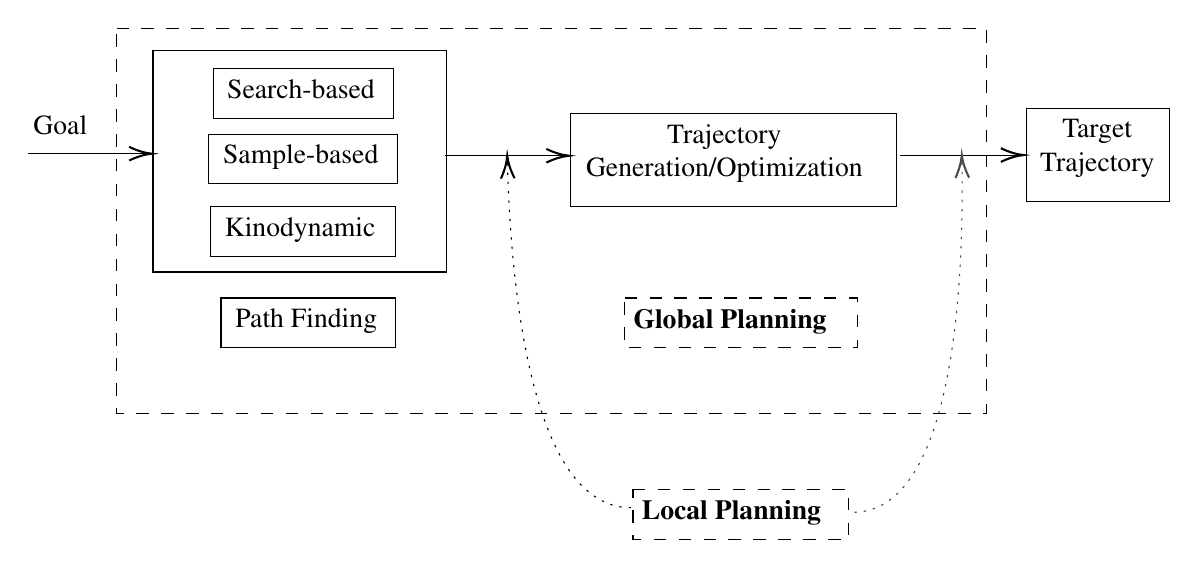
\begin{tikzpicture}[x=0.75pt,y=0.75pt,yscale=-1,xscale=1]
%uncomment if require: \path (0,267); %set diagram left start at 0, and has height of 267

%Shape: Rectangle [id:dp575866165243341] 
\draw   (89.56,19.67) -- (230.89,19.67) -- (230.89,126.44) -- (89.56,126.44) -- cycle ;
%Straight Lines [id:da8414235785777104] 
\draw    (230.44,70.44) -- (288,70.44) ;
\draw [shift={(290,70.44)}, rotate = 180] [color={rgb, 255:red, 0; green, 0; blue, 0 }  ][line width=0.75]    (10.93,-3.29) .. controls (6.95,-1.4) and (3.31,-0.3) .. (0,0) .. controls (3.31,0.3) and (6.95,1.4) .. (10.93,3.29)   ;
%Straight Lines [id:da08815651015896142] 
\draw    (29.44,69.44) -- (87,69.44) ;
\draw [shift={(89,69.44)}, rotate = 180] [color={rgb, 255:red, 0; green, 0; blue, 0 }  ][line width=0.75]    (10.93,-3.29) .. controls (6.95,-1.4) and (3.31,-0.3) .. (0,0) .. controls (3.31,0.3) and (6.95,1.4) .. (10.93,3.29)   ;
%Straight Lines [id:da22108099082080424] 
\draw    (449.44,70.11) -- (507,70.11) ;
\draw [shift={(509,70.11)}, rotate = 180] [color={rgb, 255:red, 0; green, 0; blue, 0 }  ][line width=0.75]    (10.93,-3.29) .. controls (6.95,-1.4) and (3.31,-0.3) .. (0,0) .. controls (3.31,0.3) and (6.95,1.4) .. (10.93,3.29)   ;
%Curve Lines [id:da017803972324741846] 
\draw [color={rgb, 255:red, 0; green, 0; blue, 0 }  ,draw opacity=1 ] [dash pattern={on 0.84pt off 2.51pt}]  (319.78,240) .. controls (270.94,240) and (261.74,130.66) .. (260.26,72.2) ;
\draw [shift={(260.22,70.44)}, rotate = 88.68] [color={rgb, 255:red, 0; green, 0; blue, 0 }  ,draw opacity=1 ][line width=0.75]    (10.93,-3.29) .. controls (6.95,-1.4) and (3.31,-0.3) .. (0,0) .. controls (3.31,0.3) and (6.95,1.4) .. (10.93,3.29)   ;
%Curve Lines [id:da912860022154641] 
\draw [color={rgb, 255:red, 74; green, 74; blue, 74 }  ,draw opacity=1 ] [dash pattern={on 0.84pt off 2.51pt}]  (427.56,242.22) .. controls (475.74,240.9) and (480.46,130.36) .. (479.26,71.87) ;
\draw [shift={(479.22,70.11)}, rotate = 88.68] [color={rgb, 255:red, 74; green, 74; blue, 74 }  ,draw opacity=1 ][line width=0.75]    (10.93,-3.29) .. controls (6.95,-1.4) and (3.31,-0.3) .. (0,0) .. controls (3.31,0.3) and (6.95,1.4) .. (10.93,3.29)   ;
%Shape: Rectangle [id:dp5818665047698117] 
\draw  [dash pattern={on 4.5pt off 4.5pt}] (72,9) -- (491,9) -- (491,194.5) -- (72,194.5) -- cycle ;

% Text Node
\draw    (122.33,139) -- (206.33,139) -- (206.33,163) -- (122.33,163) -- cycle  ;
\draw (125.33,143) node [anchor=north west][inner sep=0.75pt]   [align=left] {\begin{minipage}[lt]{55.15pt}\setlength\topsep{0pt}
\begin{center}
{\fontfamily{ptm}\selectfont Path Finding}
\end{center}

\end{minipage}};
% Text Node
\draw    (118.5,28.5) -- (205.5,28.5) -- (205.5,52.5) -- (118.5,52.5) -- cycle  ;
\draw (121.5,32.5) node [anchor=north west][inner sep=0.75pt]   [align=left] {\begin{minipage}[lt]{57.1pt}\setlength\topsep{0pt}
\begin{center}
{\fontfamily{ptm}\selectfont Search-based}
\end{center}

\end{minipage}};
% Text Node
\draw    (116.5,60) -- (207.5,60) -- (207.5,84) -- (116.5,84) -- cycle  ;
\draw (119.5,64) node [anchor=north west][inner sep=0.75pt]   [align=left] {\begin{minipage}[lt]{59.94pt}\setlength\topsep{0pt}
\begin{center}
{\fontfamily{ptm}\selectfont Sample-based}
\end{center}

\end{minipage}};
% Text Node
\draw    (117.33,95) -- (206.33,95) -- (206.33,119) -- (117.33,119) -- cycle  ;
\draw (120.33,99) node [anchor=north west][inner sep=0.75pt]   [align=left] {\begin{minipage}[lt]{58.25pt}\setlength\topsep{0pt}
\begin{center}
{\fontfamily{ptm}\selectfont Kinodynamic}
\end{center}

\end{minipage}};
% Text Node
\draw    (290.78,50) -- (447.78,50) -- (447.78,95) -- (290.78,95) -- cycle  ;
\draw (293.78,54) node [anchor=north west][inner sep=0.75pt]   [align=left] {\begin{minipage}[lt]{104.69pt}\setlength\topsep{0pt}
\begin{center}
{\fontfamily{ptm}\selectfont Trajectory }\\{\fontfamily{ptm}\selectfont Generation/Optimization}
\end{center}

\end{minipage}};
% Text Node
\draw (30.67,49.67) node [anchor=north west][inner sep=0.75pt]   [align=left] {{\fontfamily{ptm}\selectfont Goal}};
% Text Node
\draw    (510.33,47.67) -- (579.33,47.67) -- (579.33,92.67) -- (510.33,92.67) -- cycle  ;
\draw (513.33,51.67) node [anchor=north west][inner sep=0.75pt]   [align=left] {\begin{minipage}[lt]{44.84pt}\setlength\topsep{0pt}
\begin{center}
{\fontfamily{ptm}\selectfont Target }\\{\fontfamily{ptm}\selectfont Trajectory}
\end{center}

\end{minipage}};
% Text Node
\draw  [dash pattern={on 4.5pt off 4.5pt}]  (320.8,231.22) -- (424.8,231.22) -- (424.8,255.22) -- (320.8,255.22) -- cycle  ;
\draw (323.8,235.22) node [anchor=north west][inner sep=0.75pt]   [align=left] {{\fontfamily{ptm}\selectfont \textbf{Local Planning}}};
% Text Node
\draw  [dash pattern={on 4.5pt off 4.5pt}]  (316.8,139) -- (428.8,139) -- (428.8,163) -- (316.8,163) -- cycle  ;
\draw (319.8,143) node [anchor=north west][inner sep=0.75pt]   [align=left] {{\fontfamily{ptm}\selectfont \textbf{Global Planning}}};


\end{tikzpicture}
\end{adjustbox}
\caption{Hierarchical planning pipeline: The path-finding module 
finds a geometric collision-free path, and then trajectory
optimization module generates a state-admissable kinodynamic
feasible trajectory. Local planning methods can be 
incorporated in different stages.}
\label{fig:concept}
\end{figure}

In general, path-planning algorithms for robot navigation can be divided into two major categories: global and local methods.  
Global methods focus on finding collision-free paths from the current robot position to a global goal position mostly in static scenes, while local methods tend to reactively avoid both static and dynamic obstacles. 
In order to generate smooth trajectories for robots to follow, based on the discrete planned waypoints, the trajectory optimization module is usually added in the whole pipeline. 
The path-finding module is called the frontend and the optimization module is called the backend. 
A typical traditional path-planning pipeline can be found in Fig.~\ref{fig:concept}.

% \begin{algorithm}
\caption{A* Algorithm}
\label{alg:a_star}
\begin{algorithmic}[1]
\REQUIRE $start$: starting node, $goal$: goal node
\STATE $openSet \gets \{start\}$
\STATE $cameFrom \gets$ empty map
\STATE $gScore[start] \gets 0$
\STATE $fScore[start] \gets heuristic(start, goal)$
\WHILE{$openSet$ is not empty}
  \STATE $current \gets$ node in $openSet$ with lowest $fScore$
  \IF{$current = goal$}
    \RETURN reconstructPath($cameFrom$, $current$)
  \ENDIF
  \STATE remove $current$ from $openSet$
  \FORALL{$neighbor$ of $current$}
    \STATE $tentativeGScore \gets gScore[current] + dist(current, neighbor)$
    \IF{$neighbor$ not in $gScore$ or $tentativeGScore < gScore[neighbor]$}
      \STATE $cameFrom[neighbor] \gets current$
      \STATE $gScore[neighbor] \gets tentativeGScore$
      \STATE $fScore[neighbor] \gets gScore[neighbor] + heuristic(neighbor, goal)$
      \IF{$neighbor$ not in $openSet$}
        \STATE add $neighbor$ to $openSet$
      \ENDIF
    \ENDIF
  \ENDFOR
\ENDWHILE
\RETURN failure
\end{algorithmic}
\end{algorithm}

Global search-based algorithms such as depth-first search (DFS), breadth-first search (BFS), Dijkstra \cite{wang2011application}, and A* \cite{hart1968formal}, use path-search methods with (or without) certain pre-defined heuristics to find geometrically feasible paths on given grid maps. 
A key assumption for these methods to perform path-finding is the map is given, which can be difficult to be obtained in certain situations. 
Though these search-based methods can perform well, they can have longer search time when the space scales.
% Alg.~\ref{alg:a_star} shows the A* path-planning algorithm which returns the shortest path from the source node to the target node. 
Sample-based methods such as rapidly exploring random tree (RRT), probabilistic roadmap (PRM), and their variants use sampling in the configuration space (C-Space) to crate collision-free paths \cite{lavalle2001rapidly,karaman2011sampling,kavraki1996probabilistic}. 
% The general form of RRT and PRM algorithms can be found in Alg.~\ref{alg:rrt} and Alg.~\ref{alg:prm}, respectively.
% \begin{algorithm}
\SetAlgoLined
\KwIn{Start state $q_{start}$, goal region $G$, maximum number of iterations $K$, step size $\Delta q$, collision checking function $IsCollisionFree$, tree $T$}
\KwOut{A path from $q_{start}$ to $G$ if found, otherwise failure}
Add $q_{start}$ to $T$\;
\For{$k=1$ \KwTo $K$}{
  $q_{rand} \gets$ RandomState()\;
  $q_{near} \gets$ NearestVertex($T$, $q_{rand}$)\;
  $q_{new} \gets$ Steer($q_{near}$, $q_{rand}$, $\Delta q$)\;
  \If{!IsCollisionFree($q_{near}$, $q_{new}$)}{
    continue\;
  }
  Add $q_{new}$ to $T$\;
  \If{$q_{new} \in G$}{
    \Return Path($q_{start}$, $q_{new}$)\;
  }
}
\Return failure\;
\caption{Rapidly-Exploring Random Tree (RRT)}
\label{alg:rrt}
\end{algorithm}

% \begin{algorithm}
\SetAlgoLined
\KwIn{Start state $q_{start}$, goal state $q_{goal}$, collision checker $CC$, sample distribution $P$, number of samples $N$, number of neighbors $K$, connection distance $r$}
\KwOut{A path from $q_{start}$ to $q_{goal}$, or failure}
$V \gets \{q_{start}\}$\;
$E \gets \emptyset$\;
\For{$i \gets 1$ \KwTo $N$}{
  $q_i \gets$ sample from $P$\;
  \If{$CC(q_i)$}{
    $V \gets V \cup \{q_i\}$\;
    $Q \gets$ $K$ nearest neighbors of $q_i$ in $V$\;
    \For{$q_j \in Q$}{
      \If{$CC(q_i, q_j)$}{
        $E \gets E \cup \{(q_i, q_j)\}$\;
      }
    }
  }
}
$G \gets (V, E)$\;
\If{there is no path from $q_{start}$ to $q_{goal}$ in $G$}{
  \Return failure\;
}
$P \gets$ shortest path from $q_{start}$ to $q_{goal}$ in $G$\;
\Return $P$\;
\caption{Probabilistic Roadmap (PRM)}
\label{alg:prm}
\end{algorithm}

However, the tree nodes in these methods need to cover the whole C-Space which may suffer from heavy computational loads especially when the space is large.  
Optimization-based method such as model predictive control (MPC) added with obstacle constraints or with additional environment-related terms \cite{park2009obstacle}, \cite{ji2016path}  can be used to generate collision-free paths. 
However, MPC-related methods need to tradeoff among the length of the time horizon, the computational loads, and optimality. Short time horizon often leads the problem to sub-optimal solutions.
Both search- and sample-based methods can generate geometrically collision-free paths but possibly having great jerks (i.e., the time derivatives of the accelerations) or violating the underlying robots' dynamics.
For example, most ground vehicles are not holonomic, i.e., they cannot move freely in all directions in 2D space, where their motions are governed by their mechanical and motional constraints.

Most global methods perform well in static environments, but poorly in dynamic environments. 
Local path-planning methods can be employed to handle this problem. 
An early local obstacle-avoidance method is artificial potential field (APF) \cite{warren1989global}.
APF formulates the potentials on a given path as the inside and outside ones, and pushes the path from high-potential to low-potential region by finding the lowest potential value. 
If the waypoints on the path across the obstacle (in the obstacle), the potential is formulated as 
\begin{equation}
\label{eq:APF_in}
U_{\text{in}} = 
U_{\text{max}}(1 - \frac{R_{\text{in}}}{R_{\text{max}}}) + 
U_{\text{offset}}
\end{equation}
where $U_{\text{max}}$ is the max potential, $R_{\text{in}}$ is the distance to the centroid of the obstacle, $R_{\text{max}}$ is the max radius of the obstacle, and $U_{\text{offset}}$ is the extra potential penalty.
The outside potential is formulated as 
\begin{equation}
\label{eq:APF_out}
U_{\text{out}} = 
\frac{1}{2}U_{\text{offset}}(1+ \frac{1}{1+R_\text{out}})
\end{equation}
where $R_{\text{out}}$ is the distance outside the obstacle.
APF can be used for quadrotor path-planning \cite{chen2016uav}.
However, when multiple obstacles presented, APF can suffer from the problem of local minimum \cite{koren1991potential}.

%% Motion planning

%% trajectory generation

While path-planning algorithms can generate collision-free 2D or 3D paths or waypoints for robots, they assume a holonomic point-mass model which may result in dynamic unfeasible paths for certain non-holonomic robots, e.g., cars. 
Motion planning algorithms are considered deeply coupled with robots' kinodynamic models to generate high-dimension feasible motions (e.g., accelerations, jerks, and angular velocities). 

\subsection{RL-based Planning and Control Methods}

\subsection{Multi-robot Planning and Control}

\section{Problem Formulation}

\bibliographystyle{IEEEtran}
\bibliography{report}


\end{document}


